%%
%% This is file `uantwerpenbamathesis-example.tex',
%% generated with the docstrip utility.
%%
%% The original source files were:
%%
%% uantwerpendocs.dtx  (with options: `bmt-example')
%% 
%% This is a generated file.
%% 
%% Copyright (C) 2013-2022  by Walter Daems <walter.daems@uantwerpen.be>
%% 
%% This work may be distributed and/or modified under the conditions of
%% the LaTeX Project Public License, either version 1.3 of this license
%% or (at your option) any later version.  The latest version of this
%% license is in:
%% 
%%    http://www.latex-project.org/lppl.txt
%% 
%% and version 1.3 or later is part of all distributions of LaTeX version
%% 2005/12/01 or later.
%% 
%% This work has the LPPL maintenance status `maintained'.
%% 
%% The Current Maintainer of this work is Walter Daems.
%% 
\documentclass[we,twoside,openright,a4paper,11pt]{uantwerpenbamathesis}

\usepackage[english]{babel} % or english if your text is in English
\usepackage{pdfpages}
\usepackage[backref,hyperindex=true,pagebackref=true]{hyperref}
                          % New: you must load the hyperref package
                          % yourself! This allows you to put it in the
                          % correct order with the other packages you load!

\usepackage{mathptmx}
\iftutex
\usepackage{fontspec}
\setmainfont{Calibri} % comment this line out if you want computer
                      % modern as main font, or feel free to select
                      % any other font
\setsansfont{Calibri}
\usepackage{sansmathaccent}
\fi

\usepackage{multicol}

\bamadegree{we-en-ba-fy}

\title{Structure Analysis of Electron Beam Induced Phase Transitions in LNMO Cathodes} % either don't split titles, or do so with hypen
                     % and a newline

\author{Dylan Assinner}

\supervisor{Prof. Dr. J. Hadermann}{UAntwerpen}

\cosupervisor{S. Rahimi}{UAntwerpen}
\academicyear{2026 - 2027}


\begin{document}
\maketitle

\frontmatter

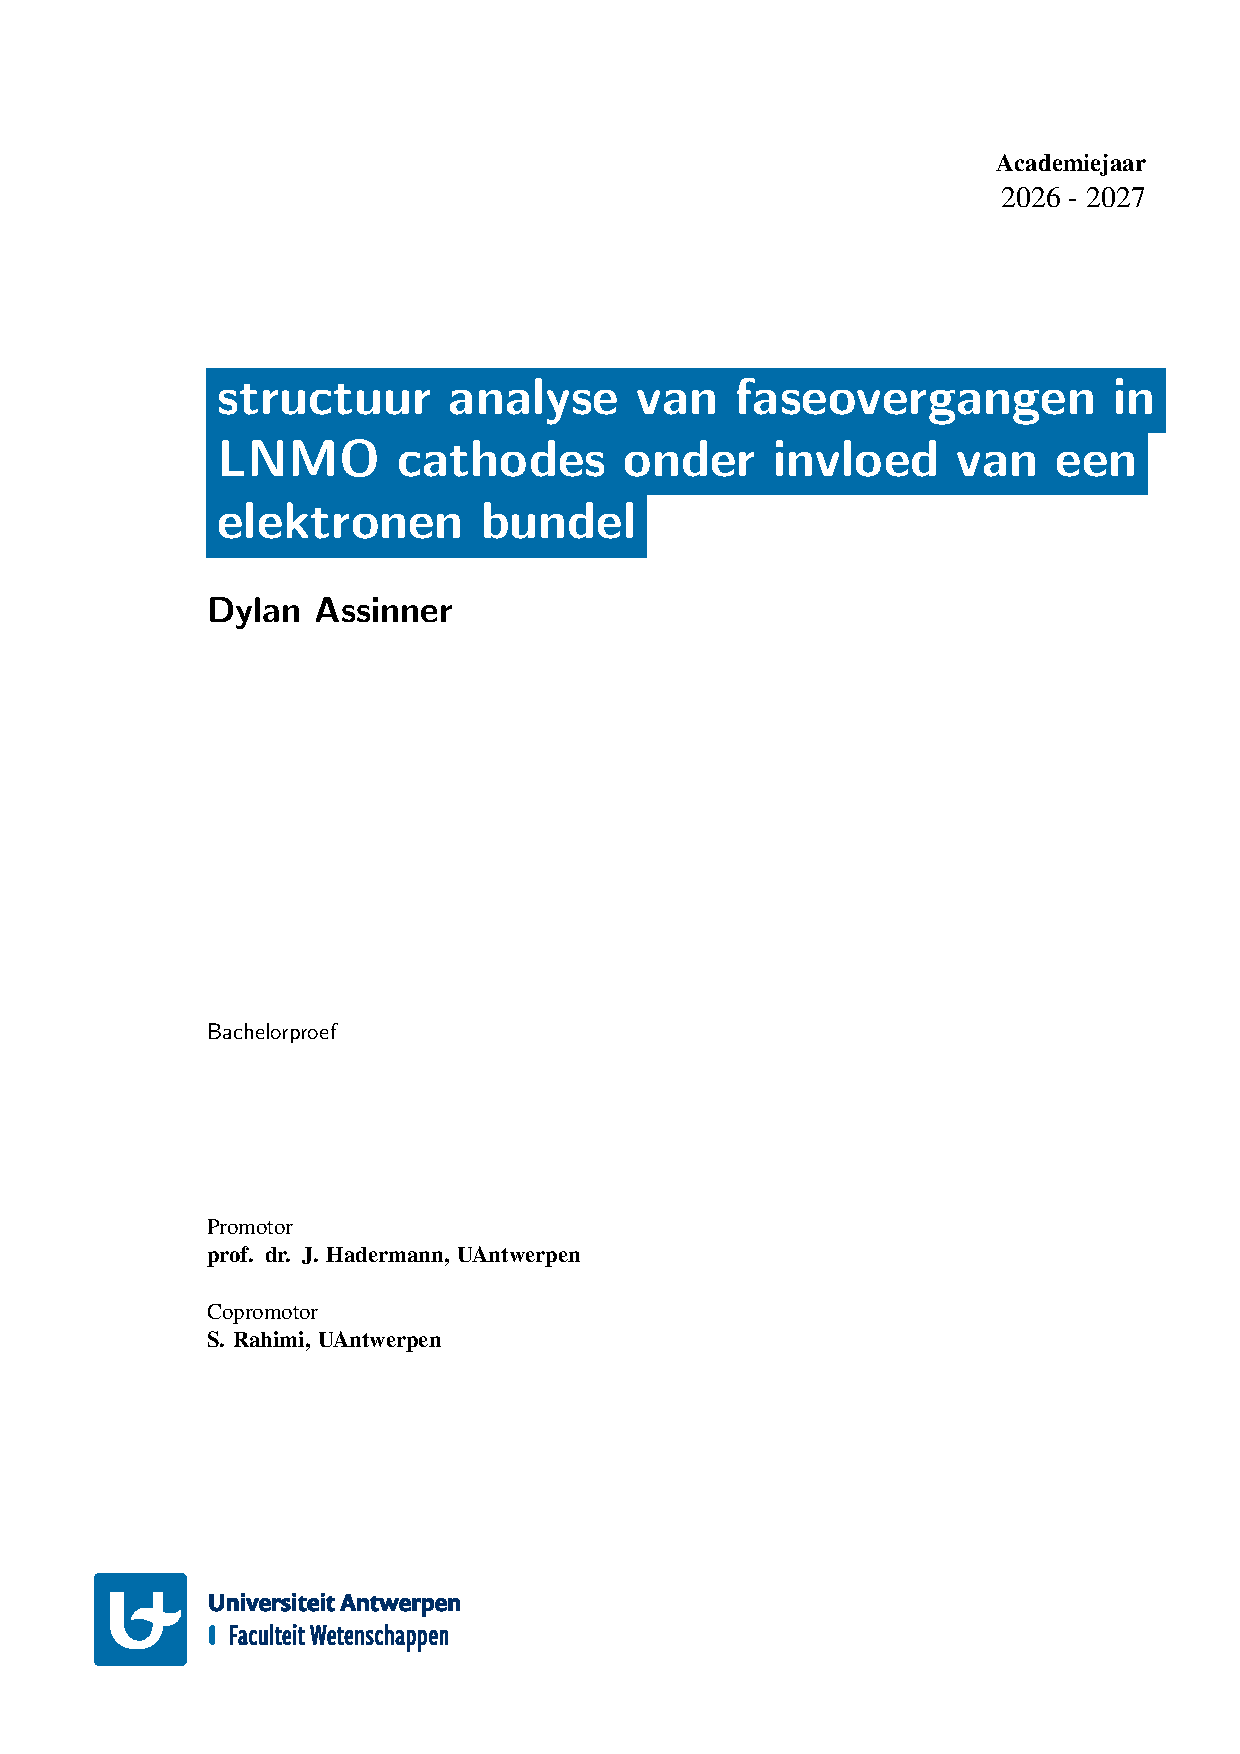
\includepdf[pages=-]{nederlands_disclaimer}9

\tableofcontents

\mainmatter

\pagestyle{empty}
\thispagestyle{empty}
\begin{multicols}{2}
	[
	\begin{center}
		\textbf{
			\Large Abstract\\[1ex]
			\@title~\\[0.5ex]}
		\@author
	\end{center}
	]
	
	\section*{English}
	\columnbreak
	\section*{Nederlands}
	
\end{multicols}

\pagestyle{fancy}


\chapter{Introduction}
\section{LNMO}
\section{3DED}
\section{4D STEM}




\chapter{Research question}

\insettext{}

\section{Procedure}

\chapter{Theoretical background}

\chapter{Results}

\chapter{Conclusion}

\appendix

\chapter{Symbols}
\chapter{References}

\end{document}


\endinput
%%
%% End of file `uantwerpenbamathesis-example.tex'.
